\chapter{Methodology}
\label{chap:methodology}

\section{Deployment Tool for an UAV Network}
\label{sec:stateoftheart:deploymenttool}

Calculating electromagnetic exposure requires knowledge about the area. The position of base stations needs to be known,
 the transmission power used by the antenna and how far the user is separated from these base stations are only a few parameters
 that have to be considered.

The WAVES research group at UGent has developed a deployment tool for disaster scenarios with the aid of UAVs \cite{J2}.
The idea of this UAV-aided emergency network is that in case of a disaster, the existing network might be damaged and will not be able 
to handle all users who are trying to reconnect to the backbone network. 
The tool makes a fast deployable network possible by attaching femtocells to UAVs, so-called \gls{UABS}s.
The tool will orchestrate the \gls{UABS}s over the disaster area. This tool is thus a suitable starting point and works as follows:

%The optimal placement for each \gls{UABS} needs to be defined to make sure that as many users as possible are properly reconnected to the backbone network while satisfying certain restrictions. 
%To make these calculations as realistic as possible the architecture of the several buildings present in the area is described in a shapefile. 
%A deployment tool calculates the optimal position of the \gls{UABS} by taking the 3D models of the building into account along with some femtocell specifications and user distribution. This deployment tool is developed by the WAVES research group, a department within Ghent University.

The deployment tool will try to calculate the optimal placement for each \gls{UABS} and requires therefore a description of the area where the UAV-aided network needs to 
be deployed. This is done with the use of so-called shape files. These files contain three dimensional descriptions of the buildings present in the area and are
key values in approaching results as realistic as possible. Furthermore, the tool also requires a time period and a configuration file containing technical specifications of the type of \gls{UABS} that is being used. 
The tool will thereafter randomly distribute users over the area and assigns a certain bitrate to them. \\
\\
In a second phase, the optimal position for each \gls{UABS} is calculated. This is done by trying to locate a \gls{UABS} above each active user. Two options are possible.
If a fixed flying height is defined, a base station is placed above each user at the given height, unless a building is obstructing its location. Then, no base station will be located above that user.
Alternatively to the fixed flying height, a flying margin can be defined which represents the distance between the outdoor user and  the drone.
If the user is inside, this margin will be measured between the drone and the rooftop of that building.
The latter is only allowed if the suggested height remains below the given maximum allowed height. \\
\\
Finally, all \gls{UABS}s are sorted on whether they were active or not, followed by the increasing path loss from each \gls{UABS} to that user.
So the algorithm starts by checking for each active \gls{UABS} if it can cover the user. If this is the case, the user will be connected to this \gls{UABS}. If not,
the second active base station with a (slightly) worse path loss is considered. If no active base station is suitable, inactive \gls{UABS}s are considered. 
The user remains uncovered if no \gls{UABS}
is found. The reason behind only considering already active base stations at first, is the high cost that comes along with each drone.
\\
Up till now, the tool has only calculated some suggestions. The actual provisioning is done in the fourth phase where drones are sorted by the amount of users they cover. As long as \gls{UABS}s
are available in the facility where they reside, \gls{UABS}s are provisioned and its users are marked as covered.

TODO: add chart/figure to support this.

%\section{Tool}
%The goals 
%\begin{figure}[h!]
%\centering
 % 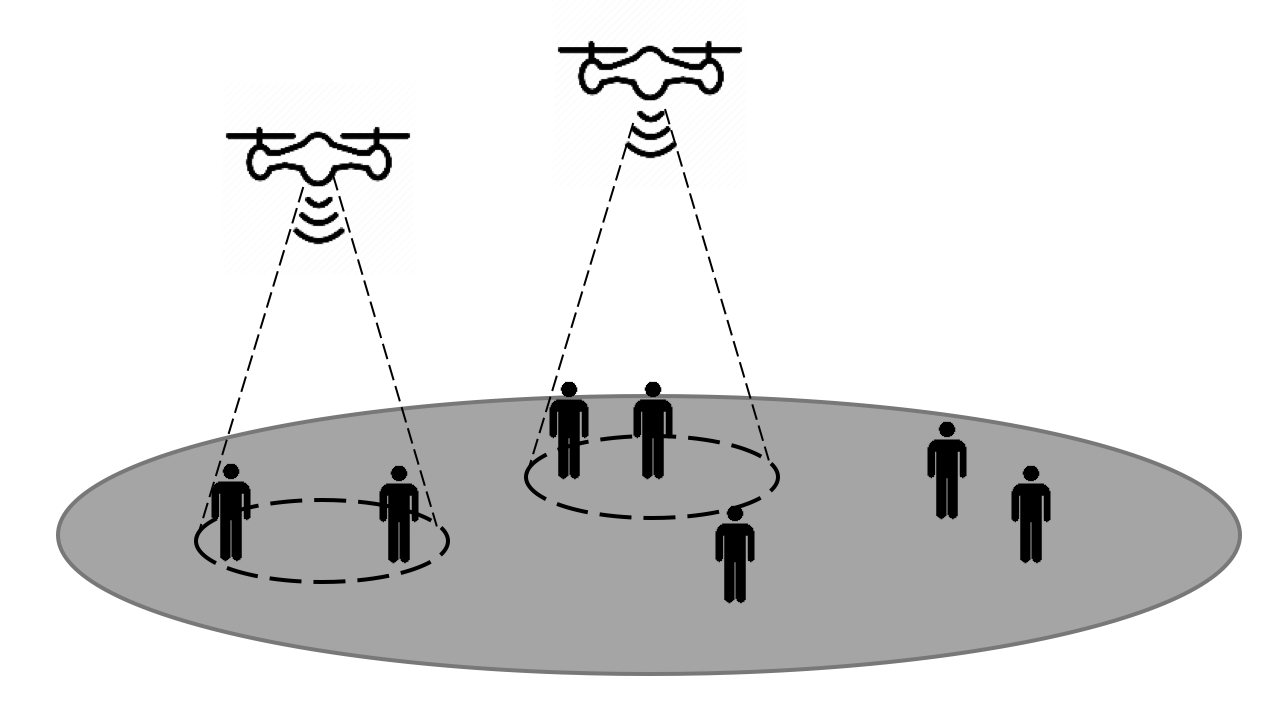
\includegraphics[width=\textwidth]{../images/generalIdeaIllustration.png}
 % \caption{Design of the microstrip patch antenna.}
 % \label{fig:antennadesign}
%\end{figure}


\section{Electromagnetic Exposure}
\subsection{Calculation of the Total Specific Absorption Rate} % (fold)
\label{sub:Calculationexposure}

The total whole body \gls{SAR} ($SAR^{wb}_{10g}$) of a user can be calculated by a simple sum of individual SAR values from the different sources.
Formula \ref{eq:overallSARwb} was originally described in \cite{J17_kuehn2019modelling} for \gls{SAR} values induced into the head.
Using $SAR^{head}_{10g}$ would however result into incorrect conclusions since 
the position of the phone relative to the user is unknown. 
The position of the phone can be next to the head but also in front of the user.
The induced electromagnetic radiation will therefore be expressed in function of the entire body.


\begin{equation} 
SAR^{wb,total}_{10g} = SAR^{wb,my_UE}_{10g} +  SAR^{wb,my_UABS}_{10g} + SAR^{wb,other_UE}_{10g} + SAR^{wb,other_UABS}_{10g}
\label{eq:overallSARwb}
\end{equation}

The first parameter, $SAR^{wb,my_UE}_{10g}$, indicates the absorbed electromagnetic radiation by the whole body originating from the user's own device. However that the 
\gls{UL} radiation is destined for the serving \gls{UABS}, a portion of that radiation is directly absorbed by its user, due to the omnidirectional nature of the mobile's antenna.
The second parameter, $SAR^{wb,my_UABS}_{10g}$, represents the \gls{DL} radiation caused by the \gls{UABS} who is serving the user.
As the third parameter, we have the $SAR^{wb,other_UE}_{10g}$ which is radiation caused by other people their device. The radiation of these devices is once again 
destinated for a specific \gls{UABS} but again, a portion of that \gls{UL} radiation will also be absorbed by our user.
Finally, $SAR^{wb,other_UABS}_{10g}$ represents the \gls{DL} radiation by the other UABSs our user is exposed to but not served by.
An illustration is given in figure \ref{fig:networkIllustration} where the green arrow is a type near field radiation while 
the others represent far field radiation. This is further 
explained is subsequent chapters along with how each value in this formula can be calculated. We can only speak in terms of \gls{SAR}
  when the electromagnetic radiation is absorbed by the user. This last step is however not shown in the illustration.

\begin{figure}[h!]
\centering
  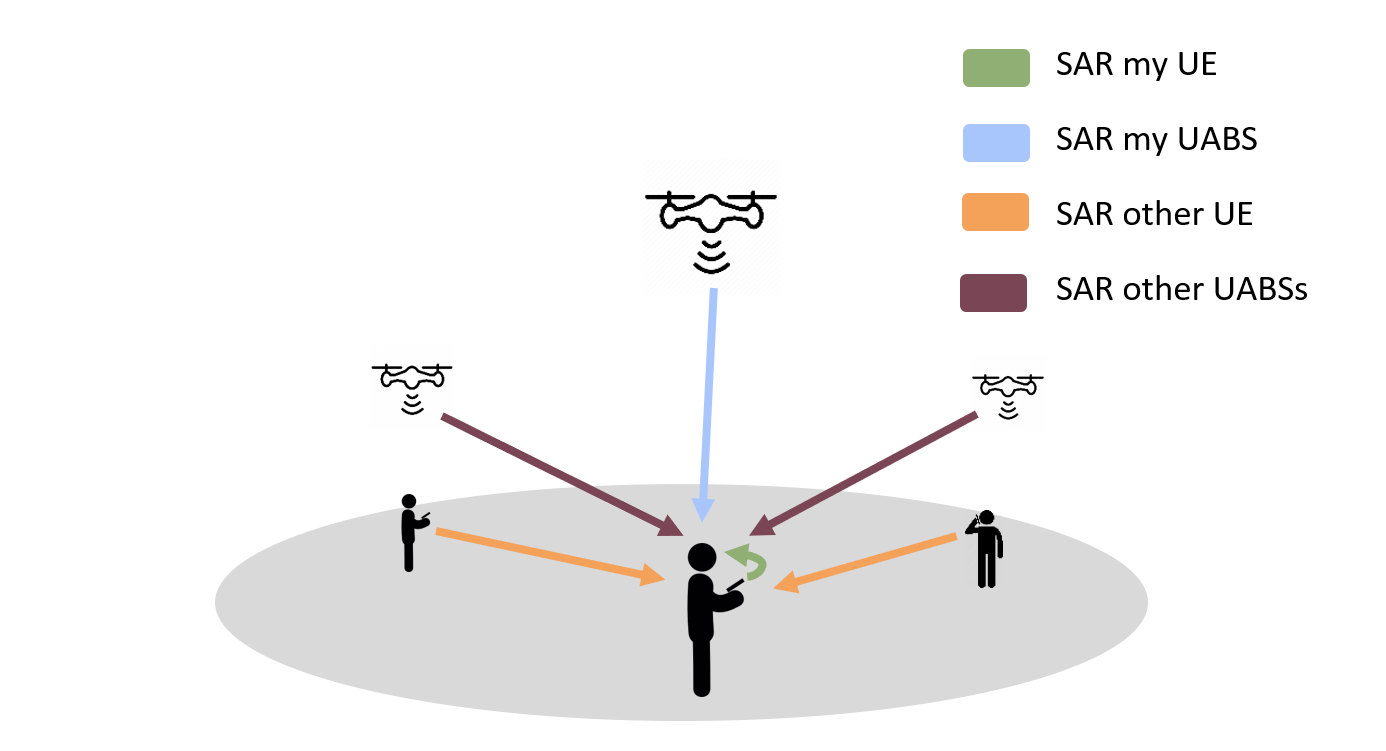
\includegraphics[width=\textwidth/3*2]{../images/networkIllustrationSARSources.png}
  \caption{Illustration of the network that shows how the average user (here shown in the center) is influenced by different type of sources. }
  \label{fig:networkIllustration}
\end{figure}

\subsection{Electromagnetic Exposure Caused by Far-Field Radiation} % (fold)
\label{sub:Calculatingdownlinkexpsure}

The electromagnetic exposure to which people are exposed can be categorized in two groups. One of them is near-field radiation which is caused 
by the user's own device and which will be discussed in \ref{sub:Uplinkexposure}.
The other type is far-field radiation and will be explained in this section. This kind of radiation is caused by radiators `far away'.
Examples of these types of radiators are \gls{UE} which belong to other people and \gls{UABS}s. 

\subsubsection{Electromagnetic Radiation from a Single Source}
\label{sec:calculatingexposure}

To determine the total exposure of a single human being or even of the entire network, the electric-field $\vec{E}$ from a single radiator $i$ should be calculated.
The formula to determine this electromagnetic value $E$ (expressed in V/m) for a specific location $u$ is given in equation \ref{eq:singleexposure}.

\begin{equation}
E_i(u) = 10^{\frac{RRP(u) - 43.15 + 20*\log(f)- PL(u)}{20}}
\label{eq:singleexposure}
\end{equation}

\paragraph{real radiation power and EIRP}
In formula \ref{eq:singleexposure}, as it was described in \cite{J6_originalExposureFormula, J1}, 
\gls{RRP} was defined as \gls{EIRP}. \gls{EIRP} is the radiation generated by an \gls{isotropicradiator} which is
a theoretical source of electromagnetic waves that radiate with the same intensity in all directions. 
The formula to find this \gls{EIRP} value (in dBm) is described in \ref{eq:eirp}
where $P_t$ stands for the input power of the antenna, $G_t$ for the gain of the transmitter and $L_t$ being its feeder loss.
\begin{equation}
EIRP = P_t + G_t - L_t
\label{eq:eirp}
\end{equation}
This formula, which is constructed out of different gains and losses, misses a factor when accounting for real life radiation patterns.
Formula \ref{eq:singleexposure} solves this by using \gls{RRP} instead of \gls{EIRP} which can be defined as follows:
\begin{equation}
RRP(u) = EIRP - attenuation(u)
\label{eq:rrp}
\end{equation}
The attenuation for a user $u$ is given based on the angle between the main beam and the user. More details on how this can be implemented is described in \ref{subsec:implementationradpat}.
When assuming that $attenuation(u)$ returns positive values, the attenuation can simply be subtracted from the EIRP-value.

\paragraph{frequency}
The used frequency in the formula above is denoted as $f$ and is expressed in MHz. Since LTE is used, this value will be 2600 MHz.

\paragraph{path loss}
\label{subsec:pl}
At last, formula \ref{eq:eirp} requires the path loss (in dB). In order to calculate this, an appropriate propagation model -of which several exist- is required .
The Walfish-Ikegami model is used since it performs well for femtocell networks in urban areas \cite{J2}. %optioneel kan je hier dezelfde bron gebruiken als dat ze in thesis van de vorige gebruikten. Bron nummer 32
It consists of two formulas depending on whether a free \gls{LOS} between the user and the base station exists or not. Both formulas expect a distance in kilometre. %bron?

\subsubsection{Combining Exposure}
The electromagnetic exposure for a given location originating from different sources can be calculated with formula \ref{eq:totalexposure} (in V/m). $E_i$ stands for 
the electromagnetic exposure from source $i$ and
$n$ stands for all far-field radiators of a certain category which will either be \gls{UABS}s or \gls{UE} from other people.
$E_{tot}$ was originally calculated for each $x$ meters \cite{J1}. In the tool, the exact location of the users is known and $E_{tot}$ will thus 
only be calculated for locations where a user is positioned.  
\begin{equation}
E_{tot} [V/m] = \sqrt{\sum_{i=1}^{n} E_i^2}
\label{eq:totalexposure}
\end{equation}

\subsubsection{Converting Far-Field Electromagnetic Exposure to $SAR^{wb}_{10g}$}
\label{sub:convertDLtosarwb}

Formula \ref{eq:overallSARwb} expects that the electromagnetic radiation is expressed into $SAR^{wb,dl}_{10g}$ and $SAR^{wb,neighbours}_{10g}$. The 
calculation for both values is in fact identical. The only difference is the source; where the first one is for \gls{UABS}s, the second one for \gls{UE}.
Physically seen, they are both whole body SAR values induced by far-field radiation ($SAR^{ff,wb}_{10g}$).

The electromagnetic radiation needs to be converted into $SAR^{ff,wb}_{10g}$. 
This conversion factor is based on Duke from the Virtual Family. Duke is a 34-year old male with a weight of 72 kg, a height of 1.74 m and body
mass index of 23.1 kg/m \cite{J22_plets2015joint}. Research shows that the conversion factor for WiFi is $0.0028 \frac{W/kg}{W/m^2}$.
 Since WiFi, at a frequency of 2400 MHz,
is very close to LTE, at 2600 MHz, it is assumed in \cite{J22_plets2015joint} that this value is also applicable for \gls{LTE}.
This constant converts the \gls{power flux density} $S$ (with units $\frac{W}{m^2}$) to the required $SAR^{ff,wb}_{10g}$.
To make this possible, the electromagnetic radiation
from formula \ref{eq:totalexposure} (expressed in  $V/m$) should first be converted to the  \gls{power flux density} with formula 
\ref{eq:flux} before formula \ref{eq:DLconvertion} can be applied.

\begin{equation}
S [W/m^2]= \frac{(E_{tot} [V/m])^2}{337}
\label{eq:flux}
\end{equation}
\begin{equation}
SAR^{wb,ff}_{10g} [W/kg]= S [W/m^2]* 0.0028
\label{eq:DLconvertion}
\end{equation}

\subsection{Electromagnetic Exposure Caused by Near-Field Radiation}
\label{sub:Uplinkexposure}
When a user is operating his device, a part of the \gls{UL} radiation will enter his body despite the fact that the 
 traffic is destined for the serving \gls{UABS}. So the 
 electromagnetic exposure will not be limited by \gls{DL} traffic from \gls{UABS}s or \gls{UL} traffic 
from other \gls{UE} but also from \gls{UL} traffic from his own device.

\subsubsection{Localized Specific Absorption Rate}

When assuming that all users hold their device next to their ear, a localized SAR-value for the head $SAR^{head}_{10g}$ can be calculated.
Various governments have defined different legislations.
The European Union uses the directions of the  \acs{IEC} who
 define in IEC:62209-2 a maximum for a 10g tissue $SAR^{head}_{10g}$ as 2 W/kg \cite{J23}.
The \acs{FCC} limits the maximum in the United States for a 1g tissue $SAR^{head}_{1g}$ at 1.6 W/kg \cite{S15_SARFCC}.
Most countries, including Belgium, enforce the 10g model and will, therefore, be the point of reference for this master dissertation.
The $SAR^{head}_{10g}$ values are phone dependent. The values reported by mobile manufactures are worst-case scenarios meaning that the 
values are measured when the phone is transmitting at maximum power. This is an understandable decision but will not result in a realistic scenario since 
modern cellular networks use power control mechanisms to prevent unnecessary high radiation of a nearby device. \gls{UE} will therefore never use more energy than 
required to maintain a connection.
To compensate for this overestimation, the actual $SAR^{head}_{10g}$ of each user will be predicted. These will, however, remain an estimation since the 
position of the phone relative to the head differs from user to user. For example, by holding the phone differently, a hand can absorb more or less 
electromagnetic radiation. The \gls{SAR} values will also depend on the age of the user, especially children who experience on average higher exposure in 
the brain regions because of different anatomical proportions \cite{J26_SARtissueage, J10_RDP}.
\begin{equation}
{SAR}_{10g}[W/kg] = \frac{P_{tx} [W]}{P^{max}_{tx} [W]} * {SAR}^{max}_{10g} [W/kg]
\label{eq:calculatesar}
\end{equation}
Equation \ref{eq:calculatesar} will be used to predict the actual $SAR^{head}_{10g}$  of a certain user with 
$P^{max}_{Tx}$ being the maximum transmission power for a phone which is in \gls{LTE} and UMTS 23 dBm \cite{J11_maxTpxUE, J10_RDP}.
The actual transmitted power ($P_{tx}$) is calculated with equation \ref{eq:ptx} where $P_{sens}$
stands for the receiver sensitivity and $PL$ the path loss between sender and receiver.
\begin{equation}
P_{tx} = P_{sens} [W] + PL [dB]
\label{eq:ptx}
\end{equation}
 
However the legal $SAR^{max}_{10g}$ for Belgium is set to $2 W/kg$,  the actual  $SAR^{max}_{10g}$ value is usually lower and different for each mobile device. 
An average is calculated based on 3516 different phones from various brands using a German database \cite{SARDatabase} for which an overview can be 
found in fig. \ref{chart:germanDatabase}.
When the phone is positioned at the ear, an average of 0.7 $W/kg$ is found with a standard deviation of 0.25 $W/kg$ which are very similar 
results as in ref. \cite{j10.1.1}.

%todo: schrijven dat het enigste verschil een std van 0.27 is?
%todo: j10.1.1 schrijft door de std van 0.25 dat er een onzekerheid van 40% is.
%todo: J10 en J10.1 rapoteert een sar max van 0.476. Update in het report is het een Nokia terwijl het bij ons voor de gemiddelde gsm is.


\definecolor{hous}{HTML}{3065c1}
\begin{figure}
  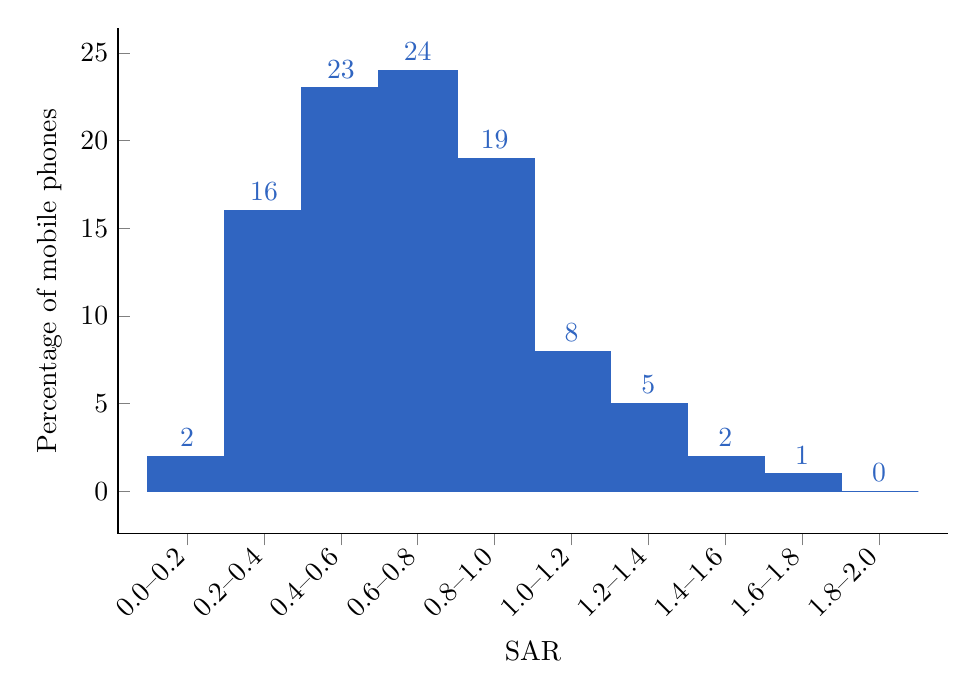
\begin{tikzpicture}
  \begin{axis}[
          ybar=-1cm,
          axis x line*=bottom,
          axis y line*=left,
          bar width=1cm,
          xlabel near ticks,
          height=8cm, width=\textwidth,
          ylabel={Percentage of mobile phones},
          xlabel={SAR},
          symbolic x coords={0.0--0.2,0.2--0.4,0.4--0.6,0.6--0.8,0.8--1.0,1.0--1.2,1.2--1.4,1.4--1.6,1.6--1.8,1.8--2.0},
          x tick label style={rotate=45, anchor=east, align=left},
          nodes near coords,
          nodes near coords align={vertical}      
          ]
          \addplot[hous,fill]  coordinates {(0.0--0.2,2)};
          \addplot[hous,fill]  coordinates {(0.2--0.4,16)};
          \addplot[hous,fill]  coordinates {(0.4--0.6,23)};
          \addplot[hous,fill]  coordinates {(0.6--0.8,24)};
          \addplot[hous,fill]  coordinates {(0.8--1.0,19)};
          \addplot[hous,fill]  coordinates {(1.0--1.2,8)};
          \addplot[hous,fill]  coordinates {(1.2--1.4,5)};
          \addplot[hous,fill]  coordinates {(1.4--1.6,2)};
          \addplot[hous,fill]  coordinates {(1.6--1.8,1)};
          \addplot[hous,fill]  coordinates {(1.8--2.0,0)};
      \end{axis}
  \end{tikzpicture}
  \caption{Distribution of how many phones belong to a certain SAR interval. Upper boundary not included.}
  \label{chart:germanDatabase}
\end{figure}


\subsubsection{Whole body Specific Absorption Rate}
The position of the phone relative to the user's body is however unknown. The tool assigns different bitrates to different phones implying 
that some users are calling and therefore probably holding their phone next to their ear while another part is using other services like browsing the web.
For this reason formula \ref{eq:overallSARwb} expects that the specific absorption rate is expressed for the entire body instead of localized $SAR^{head}_{10g}$.
The conversion factors for Duke from the Virtual Family will be used again as it was already the case in \ref{sub:convertDLtosarwb}. 
The constant to convert \gls{UL} exposure to $SAR^{wb,ul}_{10g}$
for WiFi is defined to be 0.0070 $\left(\frac{W/kg}{W}\right)$ \cite{J22_plets2015joint} which leads to eq. \ref{eq:ulToSar}.

\begin{equation} 
SAR^{wb,ul}_{10g} \left[\frac{W}{kg}\right] = 0.0070 \left[\frac{W/kg}{W}\right] * P_{tx} [W]
\label{eq:ulToSar}
\end{equation}

\section{Microstrip Patch Antenna}
\subsection{Design of  a Microstrip Patch Antenna}
\label{sub:definingAntenna}
A microstrip patch antenna is chosen because it allows easy production but more important, it has a low weight 
and has a thin profile causing it to be very aerodynamic which is useful when attaching it to a drone \cite{J13_microstripadvantages}.

The dimensions of the antenna depend on the frequency it is operating at and the characteristics of the used substrate.
The antenna will be radiating at a center frequency $f_0$ of 2.6 GHz. Each substrate has a dielectric constant $\epsilon_r$ representing 
the permittivity of the substrate and depends on the used material.
Substrates with a high dielectric constant and low height 
reduce the dimensions of the antenna
while a lower dielectric constant with a high height improves antenna performance. 
In this document, a substrate like glass 
is chosen because of the higher dielectric constant of $\epsilon_r = 4.4$ compared to materials like teflon with only a dielectric 
constant of $\epsilon_r = 2.2$ \cite{J14_antennadesign}. 
Doing this in combination with an antenna height of 2.87 mm will decrease the dimensions of the entire antenna surface.
This comes in handy since drones only have limited space available.

\begin{table}[h!]
\centering
\begin{tabular}{|l|c|l|}
\hline
 description            & symbol          & value         \\    \hline
 center frequency       & $f_0$           & 2600 Hz       \\ 
 dielectric constant    & $\epsilon_r$    & 4.4         \\ 
 heigt of the substrate & $h$             & 0.00287 m    \\ \hline
\end{tabular}
\caption{Overview of configuration parameters.}
\label{table:antennaparas}
\end{table}

The dimensions of the radiating patch can be calculated with the formulas from \cite{J14_antennadesign} and \cite{J15_antennadesign}
using the defined values from table \ref{table:antennaparas}. In that way, the width of the patch $W_{p}$ is calculated using formula \ref{eq:antennawidth}.

\begin{equation} 
W_{p} [m] = \frac{C [m/s]}{2*f_0 [Hz]}*\sqrt{\frac{\epsilon_r+1}{2}}
\label{eq:antennawidth}
\end{equation}
With $C$ being the speed of light, $f_0$ the center frequency of 2600 MHz and a dielectric constant $\epsilon_r$ of 4.4. This results 
in a width of 35.1 mm.

In order to find the length of the radiating patch, some other values need to be determined first. Formula \ref{eq:epsilonreff} will
calculate the effective dielectric constant ($\epsilon_{reff}$).
\begin{equation} 
\epsilon_{reff} = \frac{\epsilon_r+1}{2}+  \frac{\epsilon_r-1}{2} * \left(1+12*\frac{h [m]}{W_{p} [m] }\right)^{-\frac{1}{2}}
\label{eq:epsilonreff}
\end{equation}
This formula requires the width found in the previous formula along with the dielectric constant and substrate height from table \ref{table:antennaparas}.
This will result in a $\epsilon_{reff}$ of 3.91.

\begin{equation} 
L_{eff} [m] = \frac{C [m/s]}{2*f_0 [Hz]}*\sqrt{\epsilon_{reff}}
\label{eq:leff}
\end{equation}
Now formula \ref{eq:leff} can be used to calculate effective length ($L_{eff}$) which results in 29.16 mm.

\begin{equation} 
\Delta L [m]= 0.412*h*\frac{(\epsilon_{reff}+0.3)\left(\frac{W_{p} [m]}{h [m]}+0.264\right)}{\left(\epsilon_{reff}-0.258\right)\left(\frac{W_{p} [m]}{h [m]}+0.8\right)}
\label{eq:lenghtextension}
\end{equation}
Eventually, the length extension is found with formula \ref{eq:lenghtextension} by substituting the values from above.
Doing so determines that the $\Delta L$ equals 1.3071 mm.

Finally, the length of the patch can be calculated using the expression \ref{eq:realLenght}
\begin{equation} 
L_p [m]= L_{eff} [m] - 2 * \Delta L [m]
\label{eq:realLenght}
\end{equation}
The length $P_l$ results in 26.55 mm.

The dimensions of the radiation patch are now known. The only remaining questions are the dimensions of the ground plane and dielectric substrate to which the 
radiation patch is attached. The transmission line model is in fact only applicable for an infinite ground plane but it has been proven that similar results
can be achieved if the ground plane's dimensions are bigger than the patch by approximately 6 times the height of the dielectric substrate \cite{J14_antennadesign,J15_antennadesign}.

\begin{equation} 
L_{g} [m] = 6 * h [m] + L_p [m]
\end{equation}
\begin{equation} 
W_{g} [m] = 6 * h [m] + W_p [m]
\end{equation}
Therefore, the length of the ground plane $L_{g}$ should be at least 0.0438 m and a width $W_{g}$ at least 0.0524 m.
A schematic overview of how the antenna will look like is given in figure \ref{fig:antennadesign}.
\begin{figure}[h!]
\centering
  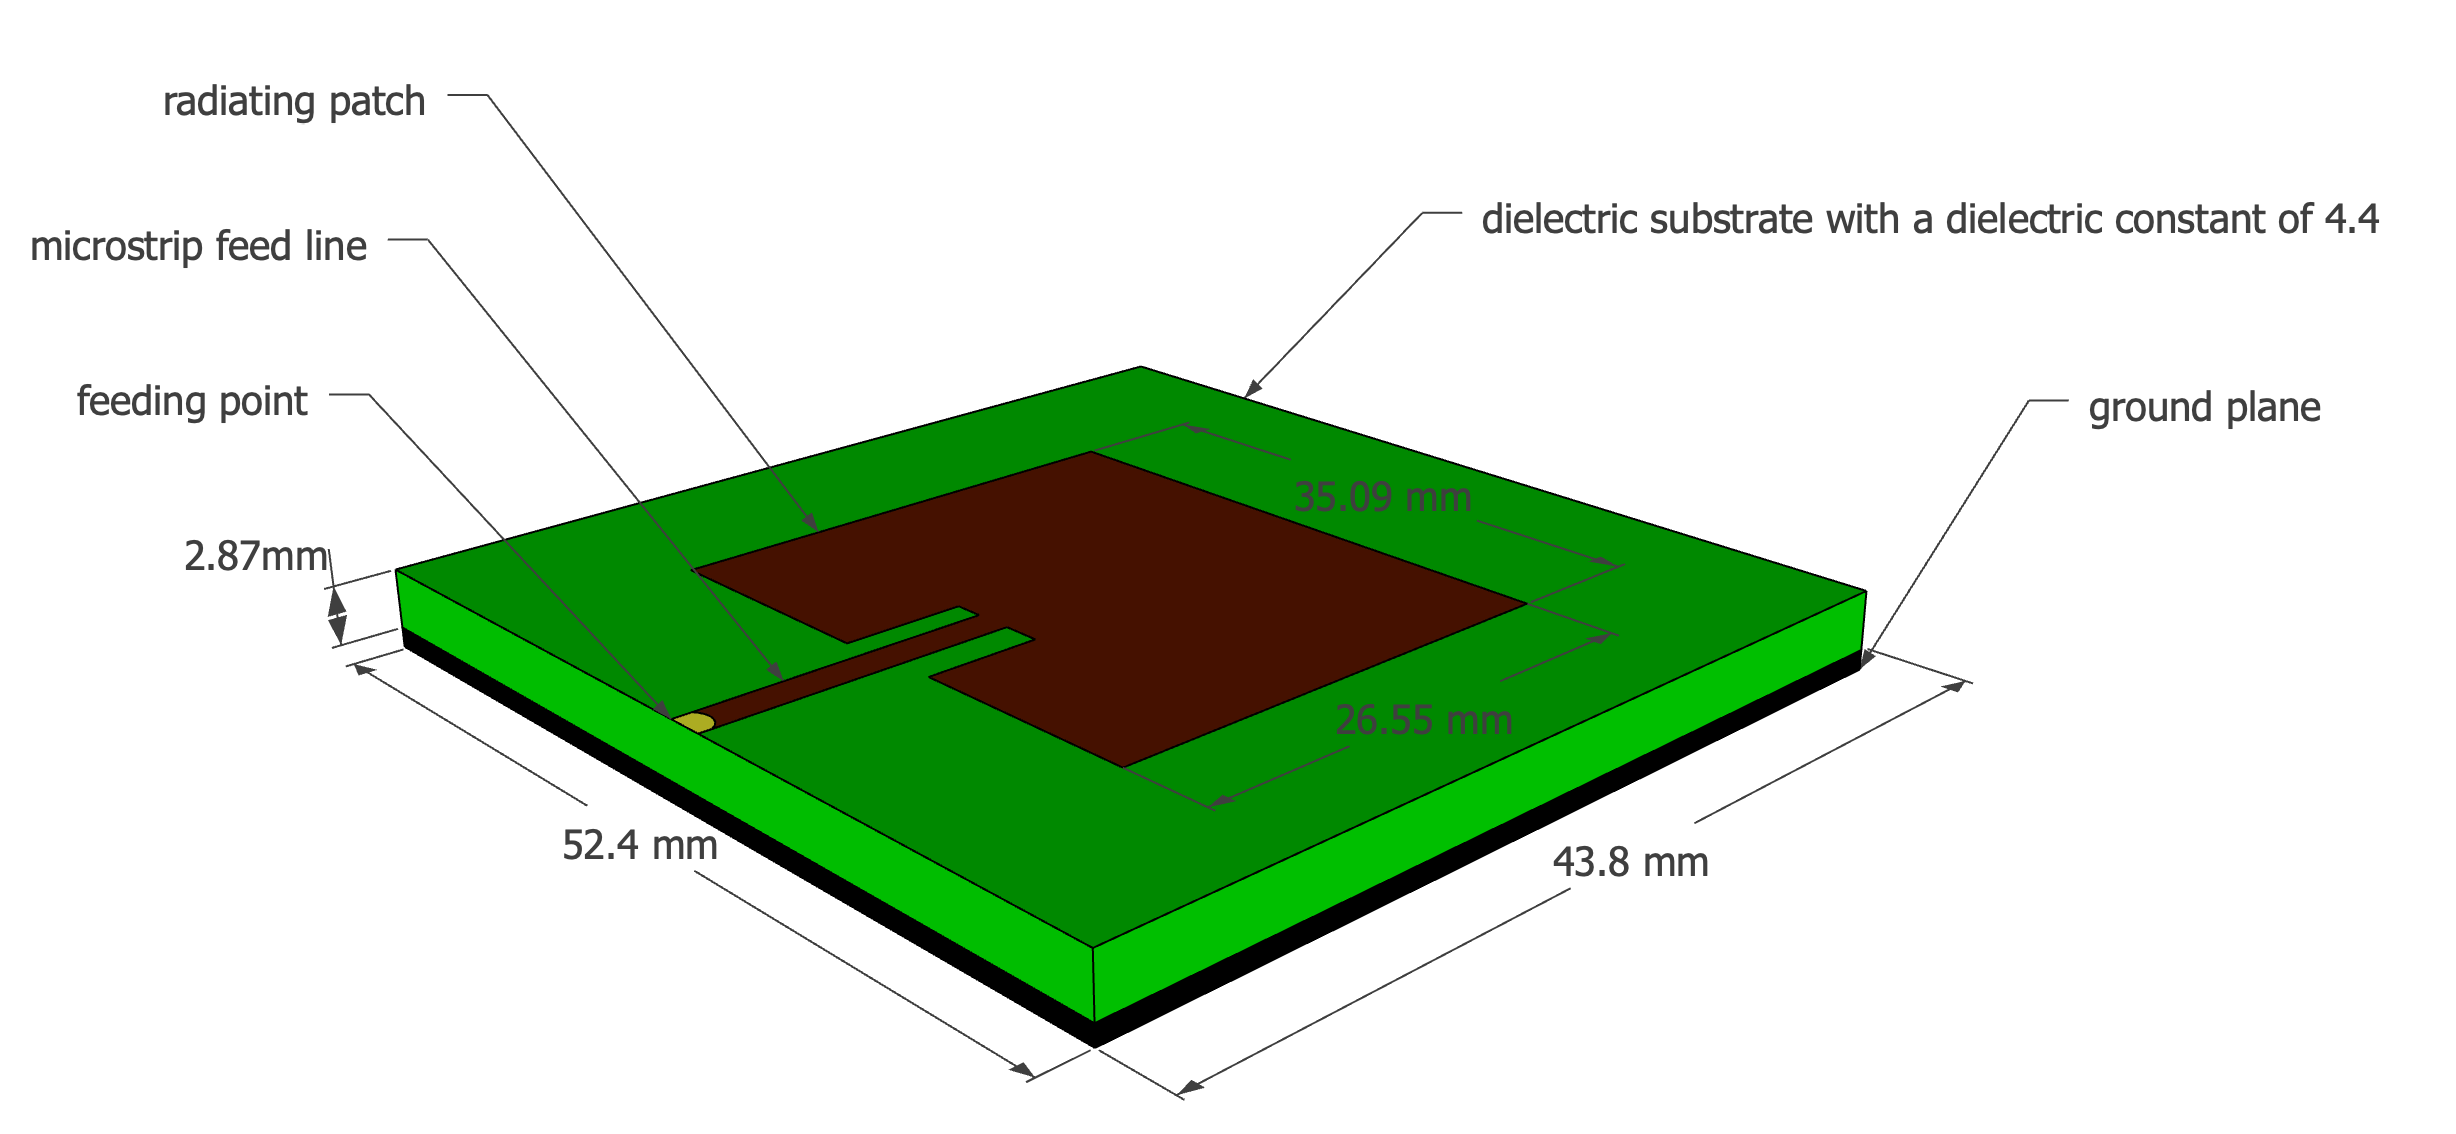
\includegraphics[width=\textwidth]{../images/MicrostripAntenna.png}
  \caption{Design of the microstrip patch antenna.}
  \label{fig:antennadesign}
\end{figure}

\subsection{Radiation Pattern}
Mathlab is able to generate the radiation pattern for this microstrip patch antenna.
The code in  listing \ref{c:mathlabradpattern} starts by defining the dielectric substrate which will be glass with a dielectric constant
of 4.4 and a height of 0.00287 m. Thereafter, the microstrip patch antenna is generated with the \verb|width| and \verb|length| being the dimensions
of the radiation patch and the \verb|GroundPlaneLength| and \verb|GroundPlaneWidth| the dimensions of the ground plane and dielectric substrate.
The \verb|FeedOffset| is the relative offset from the center where the radio frequency power is fed to the radiating patch which will here be
at the edge. This is in figure \ref{fig:antennadesign} indicated with the yellow dot. At last, the \verb|dielectric|-object is substituted into the 
\verb|patchMicrostripInsetfed|-object.

Generating the pattern is done with the \verb|pattern|-command. The first value is the \\ \verb|patchMicrostripInsetfed|-object followed by the frequency
at which the antenna will be operating. Optionally, an azimuth value can be parsed like in line 7 and 8 where 90 and 0 relatively stand for the H-plane and E-plane.

\begin{listing}[h!]
\begin{minted}[frame=single,framesep=10pt,xleftmargin=20pt,linenos]{c}
d = dielectric("Name",'glass',"Thickness",0.00287,"EpsilonR",4.4)
p = patchMicrostripInsetfed("Width",0.0351,"Length",0.02655,
    "GroundPlaneLength",0.0438,"GroundPlaneWidth",0.O524,
    "FeedOffset",[-0.021885 0],"Substrate", d)

pattern(p,2.6e9, "CoordinateSystem", 'polar', "Normalize",true)
pattern(p,2.6e9, 90, "CoordinateSystem", 'polar', "Normalize",true)
pattern(p,2.6e9, 0, "CoordinateSystem", 'polar', "Normalize",true)
\end{minted}
\caption{Mathlab code to generate radiation pattern for a microstrip patch antenna.}
\label{c:mathlabradpattern}
\end{listing}

Running the configuration from listing \ref{c:mathlabradpattern} will generate the radiation pattern from figure \ref{radpattern2}.
When running the same configuration for a slightly bigger square ground plane with an edge of 0.060 m, the radiation pattern from \ref{radpattern1} is
achieved. Both radiation patterns show an aperture angle of approximately 90°. It becomes clear that the radiation pattern from figure \ref{radpattern2} has a higher attenuation in the direction it is not facing compared to
the radiation pattern of figure \ref{radpattern1}. If it is assumed that drones fly lower than some users are positioned in some buildings, the pattern of 
\ref{radpattern1} would be a better approach. However, for the continuation of this master dissertation, the radiation pattern from figure \ref{radpattern2} 
will be used since this antenna is the smallest
and therefore more suitable to attach to the limited space available under a drone.  A data sheet of the exact values from both radiation patterns can be
found in appendix \ref{ch:radpattern}.

\begin{figure}[!htb]
\minipage{0.32\textwidth}
  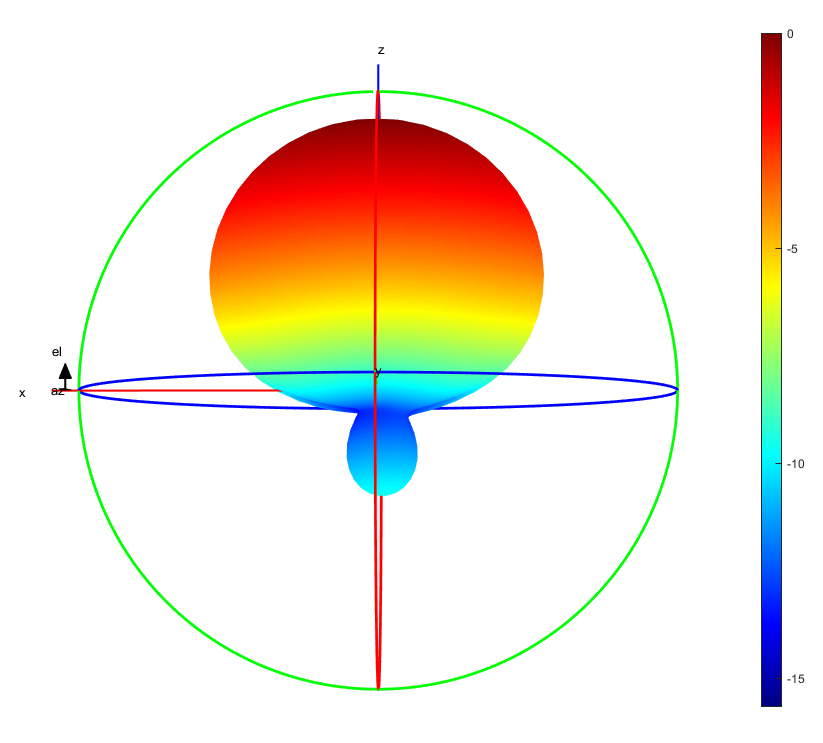
\includegraphics[width=\linewidth]{../images/pattern2/pattern.png}
\endminipage\hfill
\minipage{0.32\textwidth}
  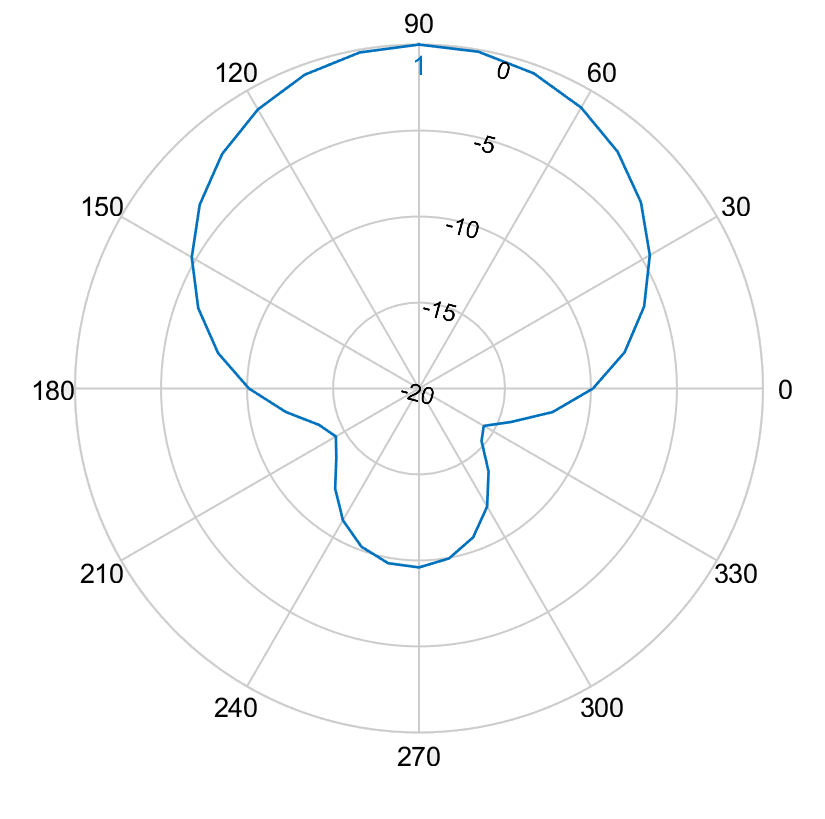
\includegraphics[width=\linewidth]{../images/pattern2/ep.png} 
\endminipage\hfill
\minipage{0.32\textwidth}%
  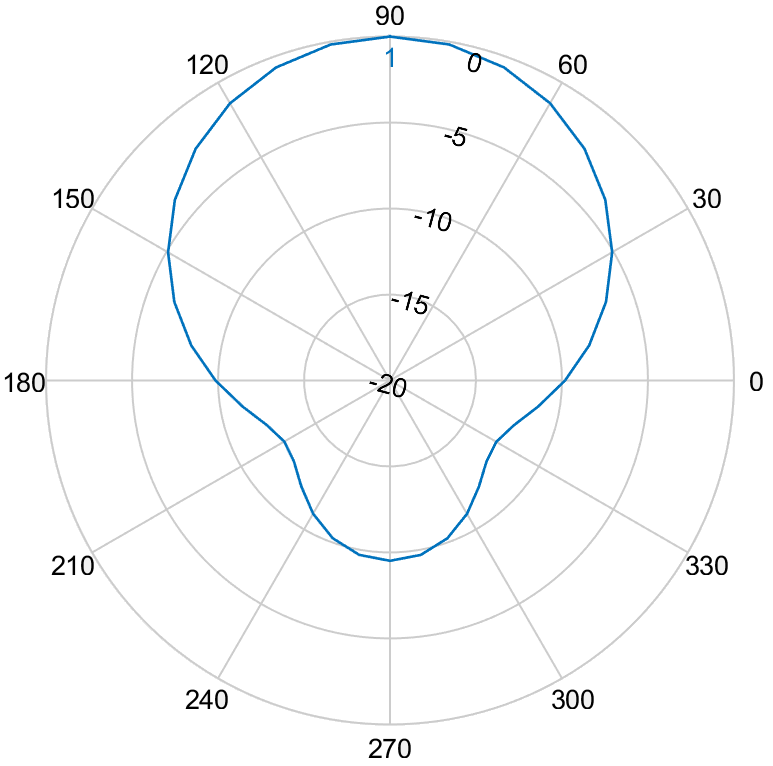
\includegraphics[width=\linewidth]{../images/pattern2/hp.png}
\endminipage
  \caption{Radiation pattern 1: On the left a 3D model of the entire pattern with the configuration as described above. In the middle a 2D radiation pattern of the E-plane and at the right a 2D model of the H-plane.}
  \label{radpattern2}
\end{figure}

\begin{figure}[!htb]
\minipage{0.32\textwidth}
  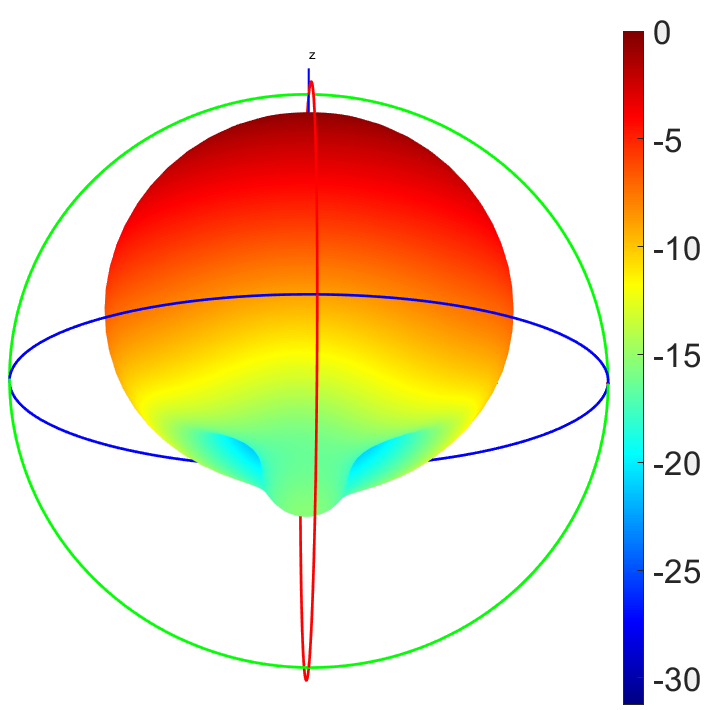
\includegraphics[width=\linewidth]{../images/pattern1/radiationPattern3D.png}
\endminipage\hfill
\minipage{0.32\textwidth}
  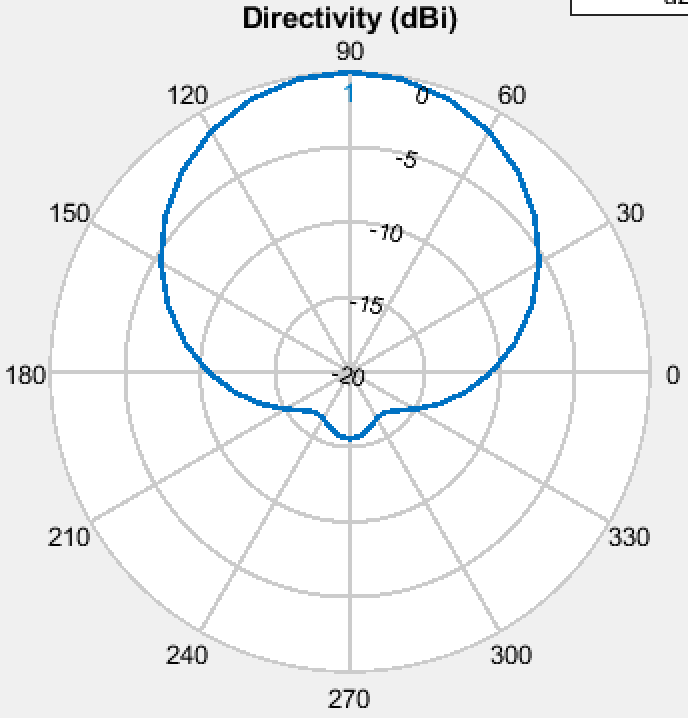
\includegraphics[width=\linewidth]{../images/pattern1/ep.png} 
\endminipage\hfill
\minipage{0.32\textwidth}%
  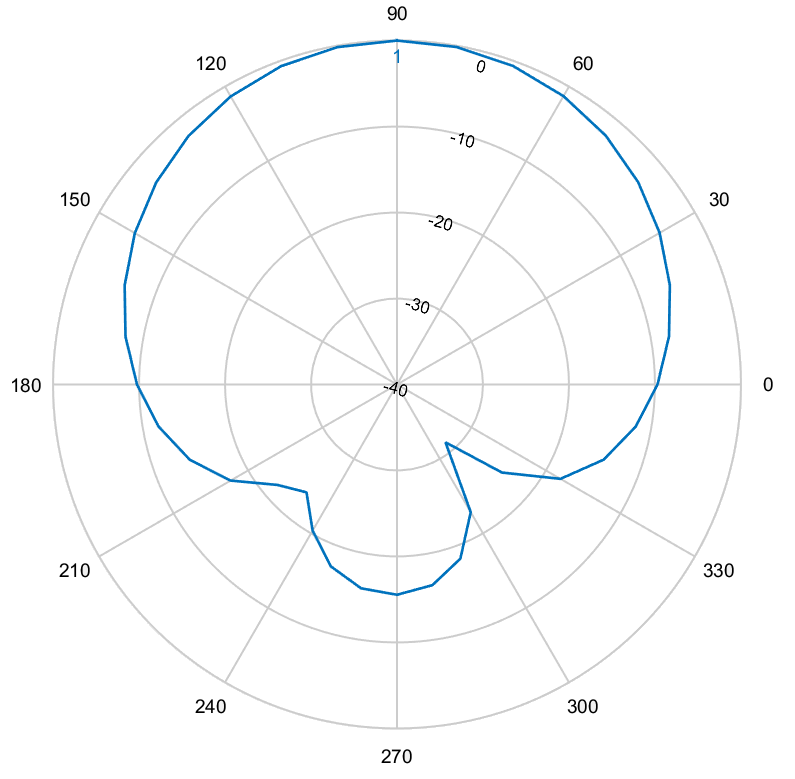
\includegraphics[width=\linewidth]{../images/pattern1/hp.png}
\endminipage
  \caption{Radiation pattern 2: Generated with a groundplane of 0.06m by 0.06m. On the left is the 3D model of the entire pattern plotted. In the middle a 2D radiation pattern of the E-plane and at the right a 2D model of the H-plane.}
 \label{radpattern1}
\end{figure}

\section{Optimizing the Network}
\label{sec:methodology:optimizingTheNetwork}

\textcolor{red}{TODO: the red paragraph belongs in this section but 
still need to check whether the text vloeit over in volgende (zwarte) paragraaf...}

 \gls{UABS}s are drones with femtocell base stations attached to it. Drones can remain in the air for only a limited time, which is certainly 
the case when also an antenna needs to be connected to the battery of his carrier. It is therefore
interesting to not only consider electromagnetic exposure of the user but also the power consumption that comes with it. 
However an increasing transmission power of an antenna comes with an increasing electromagnetic exposure. This is not the case considering
both values for an entire network. In fact, the authors from \cite{J1}  prove that both become inversely equivalent.

If a network is optimized towards power consumption, less drones will be provisioned radiating at higher power levels. This is because not only 
the transmission power is considered but also the power needed to keep the drone in the air. Therefore, it is cheaper to cover a user by 
increasing the antenna's transmission power of an already activated drone nearby as it therefore prevents the power cost of a new drone.
By increasing the transmission power, also the electromagnetic exposure will increase for users closer to that drone. An exposure optimized
network will therefore faster decide to power up a new drone.

\textcolor{red}{merge prev paragraph with the following paragraph}
The network, as originally defined in the deployment tool, tried to minimize power consumption by connecting the user to a base station which
experienced the lowest path loss. A second optimization strategy is introduced, based on the fitness function described in \cite{J1}.

\begin{equation} 
f = w * \left(1 - \frac{E_m}{E_{max}}\right) + (1 - w)*\left(1 - \frac{P}{P_{max}}\right) * 100
\label{eq:fitnessfunction}
\end{equation}

Formula \ref{eq:fitnessfunction} returns a fitness value which represents the performance of the entire network. Users are connected to different \gls{UABS}s and each time a fitness value is 
calculated. The user will eventually be connected to the drone resulting in the highest fitness value. This process is repeated for each user.
$w$ is the importance factor of electromagnetic exposure ranging from 0 to 1, boundaries included. A $w$ set to zero means that electromagnetic 
exposure is not important. Such a network will therefore be called a power consumption optimized network. 
Likewise, a $w$ set to one means that minimizing exposure is top priority and will result in an exposure optimized 
network. $P_{max}$ is the power consumption of all \gls{UABS}s, both active and inactive, when radiating at the highest possible level 
while $P$ is the effective power used by the current designed network. 
This will be the power required for the flying drones themselves and their antenna.
$E_m$ will be the weighted exposure of the average user for the current designed network and $E_{max}$ the weighted average electromagnetic exposure when all antennae are at their highest power level.

When optimizing the network, it is not only important to consider the average exposure of all users, but also to limit high extremes \cite{J1}. A weighted average 
will be used not only considering the median but also the 95 percentile from all users' \gls{DL} exposure using formula \ref{eq:em}. 
Since both values are considered to have equal importance, the weight factors $w_1$ and $w_2$ will both have an equal importance of 50\%. 

\begin{equation} 
E_m = \frac{w_1 * E_{50} + w_2 * E_{95}}{w_1 + w_2}
\label{eq:em}
\end{equation}
%\textcolor{red}{todo: in J1 is dit gedetailleerder uitgeschreven. Mogelijk om hier wat extra over te schrijven.}


\section{Implementation}

\subsection{Network Planning, Bringing It All Together}

The existing algorithm as described in section \ref{sec:stateoftheart:deploymenttool} is extended to support different optimization strategies by 
using the formulas from section \ref{sec:methodology:optimizingTheNetwork}.
As explained in State of the Art, the program starts with the preparation of the network by distributing the users over the network and assigns 
the bitrate required for each user's cell phone activity.
Thereafter, the tool tries to solve  this network by assigning a \gls{UABS} above each user. This master dissertation will only cover fixed flying heights meaning that a 
certain position is only infeasible if it is obstructed by a building.

Solving the network starts by calculating the path loss between all users and between users and \gls{UABS}s.
Thereafter, the tool iterates over each user and tries to connect that user to each \gls{UABS}. This connection is not always possible. A \gls{UABS} might be saturated with users and 
will not be able to cover yet another user or maybe the user is so far away that in order to cover that user, the \gls{UABS} would exceed its maximum allowed input power.
If however a connection is possible, the user will be connected to that \gls{UABS} and the fitness function from section \ref{sec:methodology:optimizingTheNetwork} is used. 
Only the connection which results in the best fitness value for the entire network will be used. Thereafter, the tool shifts to the next user. 

Up till now, the tool assumed an unlimited number of drones but this is an unrealistic scenario. Certainly when high number of users are present in the network.
The number of available drones can be limited by defining the capacity of the facility where the drones are stored. If such a capacity is defined and the number
of active drones exceed this limitation, the tool will delete the necessary drones starting by those who cover the least number of users. These users will now become 
uncovered.

\subsection{Implementation of the Radiation Pattern}
\label{subsec:implementationradpat}
The deployment tool originally only supported \gls{isotropicradiator}s. The tool has thus been extended and is fully configurable allowing any possible antenna 
in any possible 
orientation with the usage of a XML-file. The configuration described in this file will apply to all \gls{UABS}s. 

The orientation is done using two values called `downtilt' and `north offset'. The first value
defines the downtilt angle under wich the antenna is pointing. A downtilt angle of zero degrees is perfectly horizontal and 
an antenna with a downtilt angle of \ang{90} will be pointing straight to the ground.
This parameter only supports positive values ranging from \ang{0} to \ang{360} (upper boundary not included). An antenna pointing to the sky would therefore require a value of \ang{270}.
The second value, the north offset, defines the azimuth orientation of the drone. The value given to this parameter indicates the offset between the north
and the horizontal direction to which the antenna should be pointing at. The value once again ranges from \ang{0} to \ang{360} with the upper boundary not included. The
angle is calculated in counterclockwise orientation. For instance, a north offset of \ang{270} will let the \gls{UABS} point to the east.  

Thereafter, the normalized radiation pattern is supplied to the tool. The actual pattern is three dimensional. To simplify this,
slices perpendicular to the az-axis are extracted. These are indicated in figure \ref{fig:slicesOfPattern} with azimuth cuts. With
an angle of \ang{90} four slices are achieved, each consisting out of elevation cuts. The intersection of an elevation and azimuth plane 
corresponds with a certain attenuation which is fed to the tool. Figure \ref{fig:slicesOfPattern} shows only 3 elevation planes. The radiation pattern used in the tool 
has an attenuation every \ang{10}. In other words, a slice consists of 19 values ranging from \ang{0} to \ang{180} (boundaries included).

\begin{figure}[H]
\centering
  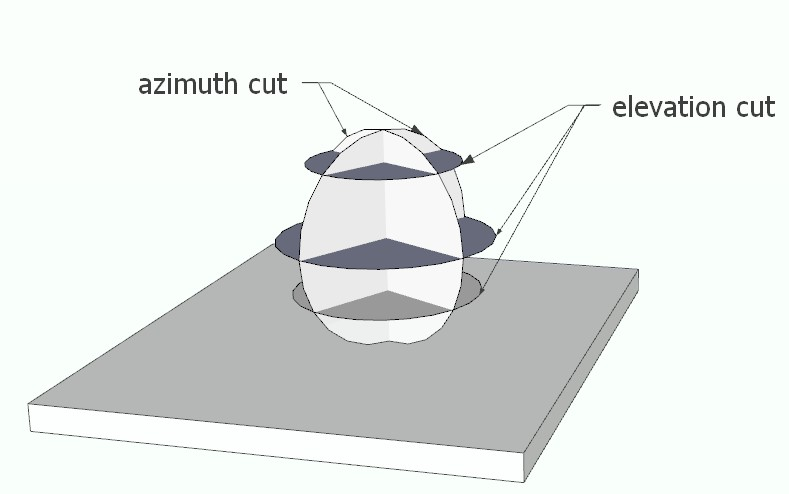
\includegraphics[width=\textwidth/3*2]{../images/3Dimages/slicesOfPattern.jpg}
  \caption{Schematic example of slices in a radiation pattern.}
  \label{fig:slicesOfPattern}
\end{figure}

The number of required slices depends on the complexity of the radiation pattern. For symmetrical radiation patterns, like 
in figure \ref{radpattern2} and \ref{radpattern1}, two azimuth cuts perpendicular to each other dividing the radiation pattern in 4 azimuth-slices 
are definitely sufficient. However, this might not be the case for radiation patterns with a more complex structure containing several  
side lobs. To tackle this issue, more azimuth-slices can be defined for increased precision. Each slice should however contain an equal amount 
of elevation slices.  A concrete example of a configuration file can be found in appendix \ref{ch:radpatexampleconfig}.
 
When the attenuation of a user from a certain \gls{UABS} needs to be known, the elevation and azimuth angles between the user and the antenna's direction 
should be calculated. 
Figure \ref{fig:globe} represents a radiation pattern with the black dot indicating the user whose attenuation needs to be calculated.
The small black lines represent azimuth and elevation planes. 
The tool knows the exact attenuation only at the intersection of those lines. 
The chance that a user is positioned at such an intersection is very small. Therefore, the attenuation for the requested point has to be estimated using bilinear interpolation.
First, the attenuation is estimated at the intersection of the red and orange line using linear interpolation on the horizontal axis with the known values at the end of the red line. 
The same is done for the orange-green intersection using the known values at the end of the green line. Finally, linear interpolation
is applied to the y-axis for the black dot on the orange line using the estimated values at the end of the orange line.

\begin{figure}[H]
\centering
  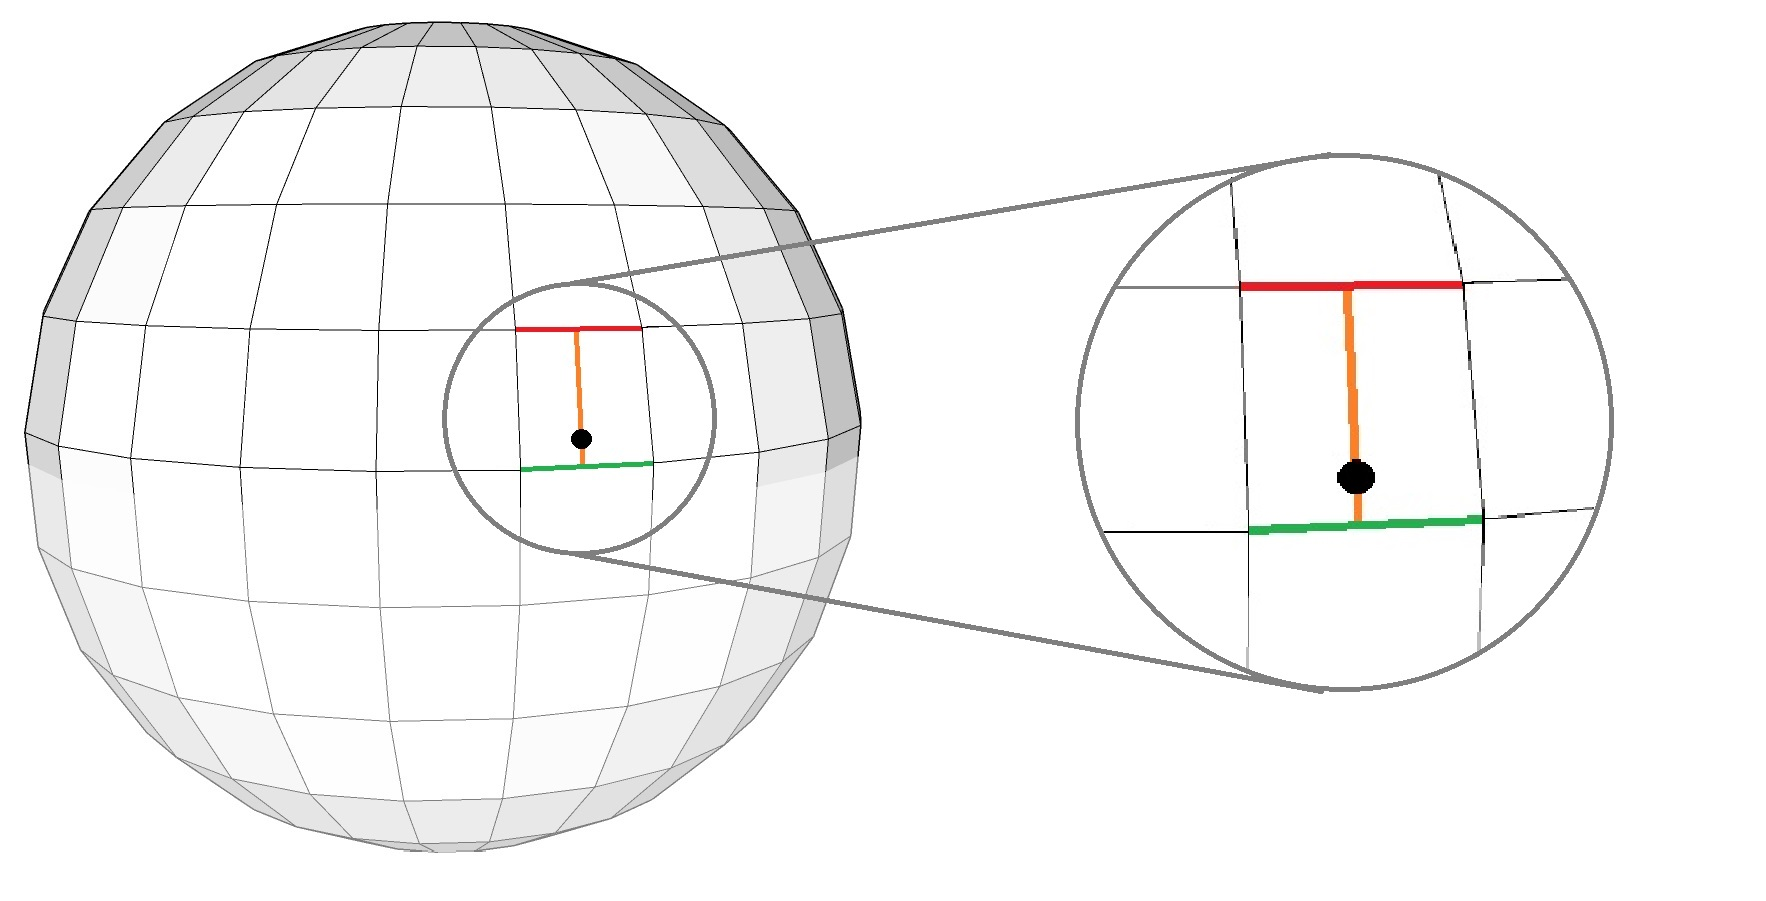
\includegraphics[width=\textwidth/3*2]{../images/3Dimages/globev2.jpg}
  \caption{Schematic example of how bilinear interpolation works.}
  \label{fig:globe}
\end{figure}

\subsection{Performance Improvement}
\subsubsection{Calculating Path Loss}
The path loss is required by several formulas. For instance, the formula that decides whether a \gls{UABS} is feasible for a certain 
user makes usage of this parameter but also the calculations for the downlink electromagnetic 
exposure require this value to be known. The formulas for the whole body $SAR_{10g}$ require not only the path loss between the user
and all \gls{UABS}s but even the path loss between users themselves. These path loss calculations are based on the Walfish-Ikegami 
model that causes a high computational load.  The calculation between two points is completely independent of any other calculation between any 
other points and is therefore a suitable candidate to multithread.
 The deployment tool creates two thread pools.
The first pool creates a thread for each user where each thread calculates the path loss between the user assigned to him and all possible \gls{UABS}s,
causing a time complexity of $n^2$.
Each user stores all path losses between himself and any other \gls{UABS}. This results therefore in a total space complexity of $n^2$.
When all users are finished, the thread pool is shut down and the second one is created for the same calculations but between users.
The pool will, just like the previous, create threads for each user but there is an important difference.
When a certain user calculates the path loss to another user, this path loss also applies for the other direction. The tool saves time by calculating the path loss only 
once and stores the path loss at both users. It is therefore sufficient that a given user only calculates path losses of users at his right side, since the other path losses will 
be calculated by the users on his left. This results in a time complexity of only $n(\frac{n}{2})$. When the last user finishes his thread, all users know the path loss of all other users causing 
a space complexity of $n(n-1)$.
% eventueel nog over concurrent hashmap

\subsubsection{Limiting Antenna Searching}
The user needs to be connected to the `best' base station. To identify this best \gls{UABS}, the user should be connected 
to each base station and the fitness value \ref{eq:fitnessfunction} of the network has to be evaluated. The connection that resulted in the best fitness function
will be added to the solution. This process is repeated for each user but can further be improved. A user will likely be connected to either the
\gls{UABS} directly above him or to a \gls{UABS} in the direct neighbourhood. Time complexity can thus be improved by not considering drones 
outside a certain radius.
An ideal data structure for neighbourhood-search is a KD-tree. This data structure is based on a binary tree and is optimal for objects with 
multiple keys. Objects are thus positioned in K dimensions where each node splits the hyperplane over exact one dimension. The dimension that needs 
to be split depends on the level of the KD-tree in which that node is situated.
In this case, the x and y coordinate will be used in a 2D-tree (k=2) like in figure \ref{fig:exampleKDtree}.

\begin{figure}[]
  \centering
  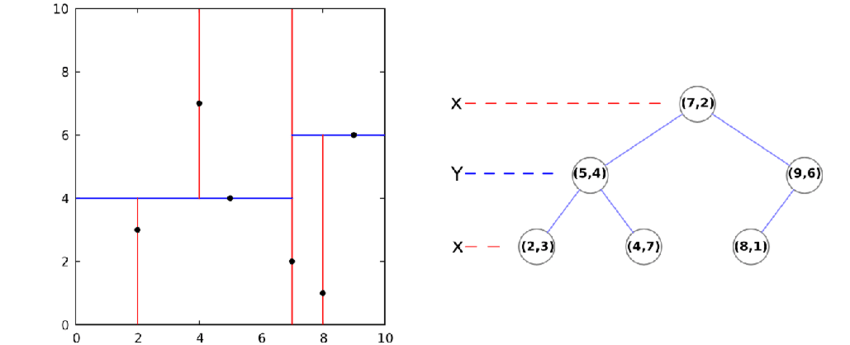
\includegraphics[width=\textwidth]{../images/Example-of-a-2D-k-d-tree.png}
  \caption{Example of a KD-tree in two dimensions.}
  \label{fig:exampleKDtree}
\end{figure}

In this case the choice was made to only consider \gls{UABS}s within a radius of half a kilometre. 
This will result in 23 \gls{UABS}s on average when applied to a default scenario of 224 \gls{UABS}s at a flying altitude of 100 m.